\documentclass[ucs,9pt]{beamer}

% Copyright 2004 by Till Tantau <tantau@users.sourceforge.net>.
%
% In principle, this file can be redistributed and/or modified under
% the terms of the GNU Public License, version 2.
%
% However, this file is supposed to be a template to be modified
% for your own needs. For this reason, if you use this file as a
% template and not specifically distribute it as part of a another
% package/program, I grant the extra permission to freely copy and
% modify this file as you see fit and even to delete this copyright
% notice.
%
% Modified by Tobias G. Pfeiffer <tobias.pfeiffer@math.fu-berlin.de>
% to show usage of some features specific to the FU Berlin template.

\usepackage[utf8x]{inputenc}
\usepackage[english]{babel}
\usepackage{arev,t1enc}
% Template for talks using the Corporate Design of the Freie Universitaet
%   Berlin, created following the guidelines on www.fu-berlin.de/cd by
%   Tobias G. Pfeiffer, <tobias.pfeiffer@math.fu-berlin.de>
% This file can be redistributed and/or modified in any way you like.
%   If you feel you have done significant improvements to this template,
%   please consider providing your modified version to
%   https://www.mi.fu-berlin.de/w/Mi/BeamerTemplateCorporateDesign

\usepackage{amsmath,dsfont,listings}

%%% FU logo
% small version for upper right corner of normal pages
\pgfdeclareimage[height=0.9cm]{university-logo}{FULogo_RGB}
\logo{\pgfuseimage{university-logo}}
% large version for upper right corner of title page
\pgfdeclareimage[height=1.085cm]{big-university-logo}{FULogo_RGB}
\newcommand{\titleimage}[1]{\pgfdeclareimage[height=2.92cm]{title-image}{#1}}
\titlegraphic{\pgfuseimage{title-image}}
%%% end FU logo

% NOTE: 1cm = 0.393 in = 28.346 pt;    1 pt = 1/72 in = 0.0352 cm
\setbeamersize{text margin right=3.5mm, text margin left=7.5mm}  % text margin

% colors to be used
\definecolor{text-grey}{rgb}{0.45, 0.45, 0.45} % grey text on white background
\definecolor{bg-grey}{rgb}{0.66, 0.65, 0.60} % grey background (for white text)
\definecolor{fu-blue}{RGB}{0, 51, 102} % blue text
\definecolor{fu-green}{RGB}{153, 204, 0} % green text
\definecolor{fu-red}{RGB}{204, 0, 0} % red text (used by \alert)

% switch off the sidebars
% TODO: loading \useoutertheme{sidebar} (which is maybe wanted) also inserts
%   a sidebar on title page (unwanted), also indents the page title (unwanted?),
%   and duplicates the navigation symbols (unwanted)
\setbeamersize{sidebar width left=0cm, sidebar width right=0mm}
\setbeamertemplate{sidebar right}{}
\setbeamertemplate{sidebar left}{}
%    XOR
% \useoutertheme{sidebar}

% frame title
% is truncated before logo and splits on two lines
% if neccessary (or manually using \\)
\setbeamertemplate{frametitle}{%
    \vskip-30pt \color{text-grey}\large%
    \begin{minipage}[b][23pt]{80.5mm}%
    \flushleft\insertframetitle%
    \end{minipage}%
}

%%% title page
% TODO: get rid of the navigation symbols on the title page.
%   actually, \frame[plain] *should* remove them...
\setbeamertemplate{title page}{
% upper right: FU logo
\vskip2pt\hfill\pgfuseimage{big-university-logo} \\
\vskip6pt\hskip3pt
% title image of the presentation
\begin{minipage}{11.6cm}
\hspace{-1mm}\inserttitlegraphic
\end{minipage}

% set the title and the author
\vskip14pt
\parbox[top][1.35cm][c]{11cm}{\color{text-grey}\inserttitle \\ \small \insertsubtitle}
\vskip11pt
\parbox[top][1.35cm][c]{11cm}{\small \insertauthor \\ \insertinstitute \\[3mm] \insertdate}
}
%%% end title page

%%% colors
\usecolortheme{lily}
\setbeamercolor*{normal text}{fg=black,bg=white}
\setbeamercolor*{alerted text}{fg=fu-red}
\setbeamercolor*{example text}{fg=fu-green}
\setbeamercolor*{structure}{fg=fu-blue}

\setbeamercolor*{block title}{fg=white,bg=black!50}
\setbeamercolor*{block title alerted}{fg=white,bg=black!50}
\setbeamercolor*{block title example}{fg=white,bg=black!50}

\setbeamercolor*{block body}{bg=black!10}
\setbeamercolor*{block body alerted}{bg=black!10}
\setbeamercolor*{block body example}{bg=black!10}

\setbeamercolor{bibliography entry author}{fg=fu-blue}
% TODO: this doesn't work at all:
\setbeamercolor{bibliography entry journal}{fg=text-grey}

\setbeamercolor{item}{fg=fu-blue}
\setbeamercolor{navigation symbols}{fg=text-grey,bg=bg-grey}
%%% end colors

%%% headline
\setbeamertemplate{headline}{
\vskip4pt\hfill\insertlogo\hspace{3.5mm} % logo on the right

\vskip6pt\color{fu-blue}\rule{\textwidth}{0.4pt} % horizontal line
}
%%% end headline

%%% footline
\newcommand{\footlinetext}{\insertshortinstitute, \insertshorttitle, \insertshortdate}
\setbeamertemplate{footline}{
\vskip5pt\color{fu-blue}\rule{\textwidth}{0.4pt}\\ % horizontal line
\vskip2pt
\makebox[123mm]{\hspace{7.5mm}
\color{fu-blue}\footlinetext
\hfill \raisebox{-1pt}{\usebeamertemplate***{navigation symbols}}
\hfill \insertframenumber}
\vskip4pt
}
%%% end footline

%%% settings for listings package
\lstset{extendedchars=true, showstringspaces=false, basicstyle=\footnotesize\sffamily, tabsize=2, breaklines=true, breakindent=10pt, frame=l, columns=fullflexible}
\lstset{language=Java} % this sets the syntax highlighting
\lstset{mathescape=true} % this switches on $...$ substitution in code
% enables UTF-8 in source code:
\lstset{literate={ä}{{\"a}}1 {ö}{{\"o}}1 {ü}{{\"u}}1 {Ä}{{\"A}}1 {Ö}{{\"O}}1 {Ü}{{\"U}}1 {ß}{\ss}1}
%%% end listings

% beamer options
\titleimage{fu_500}
\title[Spatial Databases -- Projekt]{Visualizing Results of the General Election in Germany 2013  Spatial Databases  Prof. Dr. Agnes Voisard}
\author{Alexander D\"umont \and Martin Liesenberg}
\institute[FU Berlin]{Freie Universität Berlin}
\renewcommand{\footlinetext}{\insertshortinstitute, \insertshorttitle, \insertshortdate}
\usenavigationsymbolstemplate{}
\setbeamertemplate{bibliography item}[text]

% tikz options
\usepackage{tikz-er2}
%https://bitbucket.org/pavel_calado/tikz-er2/raw/da9f9f7f169647cad6d91df7975400b1605ae67a/tikz-er2.sty
\usetikzlibrary{positioning}
\usetikzlibrary{shadows}
\tikzstyle{every entity} = [top color=white, bottom color=blue!30, 
                            draw=blue!50!black!100, drop shadow]
\tikzstyle{every weak entity} = [drop shadow={shadow xshift=.7ex, 
                                 shadow yshift=-.7ex}]
\tikzstyle{every attribute} = [top color=white, bottom color=yellow!20, 
                               draw=yellow, node distance=1cm, drop shadow]
\tikzstyle{every relationship} = [top color=white, bottom color=red!20, 
                                  draw=red!50!black!100, drop shadow]
\tikzstyle{every isa} = [top color=white, bottom color=green!20, 
                         draw=green!50!black!100, drop shadow]

% lstlisting options
\usepackage{listings}
\usepackage{color}

\definecolor{mymauve}{rgb}{0.58,0,0.82}
\definecolor{mygray}{rgb}{0.5,0.5,0.5}

\lstdefinelanguage{JavaScript}{
     keywords={var},
     keywordstyle=\color{purple}\bfseries,
     ndkeywords={d3, geo, mercator, center, scale, translate},
     ndkeywordstyle=\color{mymauve}\slshape,
     identifierstyle=\color{black},
     sensitive=false,
     comment=[l]{//},
     commentstyle=\color{green}\ttfamily,
     stringstyle=\color{red}\ttfamily
  }

\lstset{ %
  backgroundcolor=\color{white},   % choose the background color; you must add \usepackage{color} or \usepackage{xcolor}
  basicstyle=\footnotesize,        % the size of the fonts that are used for the code
  breakatwhitespace=false,         % sets if automatic breaks should only happen at whitespace
  breaklines=true,                 % sets automatic line breaking
  captionpos=b,                    % sets the caption-position to bottom
  extendedchars=true,              % lets you use non-ASCII characters; for 8-bits encodings only, does not work with UTF-8
  frame=single,                    % adds a frame around the code
  keepspaces=true,                 % keeps spaces in text, useful for keeping indentation of code (possibly needs columns=flexible)
  language=JavaScript,             % the language of the code
  numbers=left,                    % where to put the line-numbers; possible values are (none, left, right)
  numbersep=5pt,                   % how far the line-numbers are from the code
  numberstyle=\small\color{mygray}, % the style that is used for the line-numbers
  rulecolor=\color{black},         % if not set, the frame-color may be changed on line-breaks within not-black text (e.g. comments (green here))
  showspaces=false,                % show spaces everywhere adding particular underscores; it overrides 'showstringspaces'
  showstringspaces=false,          % underline spaces within strings only
  showtabs=false,                  % show tabs within strings adding particular underscores
  stepnumber=1,                    % the step between two line-numbers. If it's 1, each line will be numbered
  stringstyle=\color{mymauve},     % string literal style
  tabsize=2,                       % sets default tabsize to 2 spaces
  title=\lstname                   % show the filename of files included with \lstinputlisting; also try caption instead of title
}


\AtBeginSection[]
{
  \begin{frame}<beamer>{Outline}
    \tableofcontents[currentsection,currentsubsection]
  \end{frame}
}

\begin{document}

\begin{frame}[plain]
  \titlepage
\end{frame}

\begin{frame}{Outline}
  \tableofcontents
\end{frame}

\section{Einleitung}
\begin{frame}{Bundestagswahl 2013}
	\begin{figure}[hbtp]
		\centering
		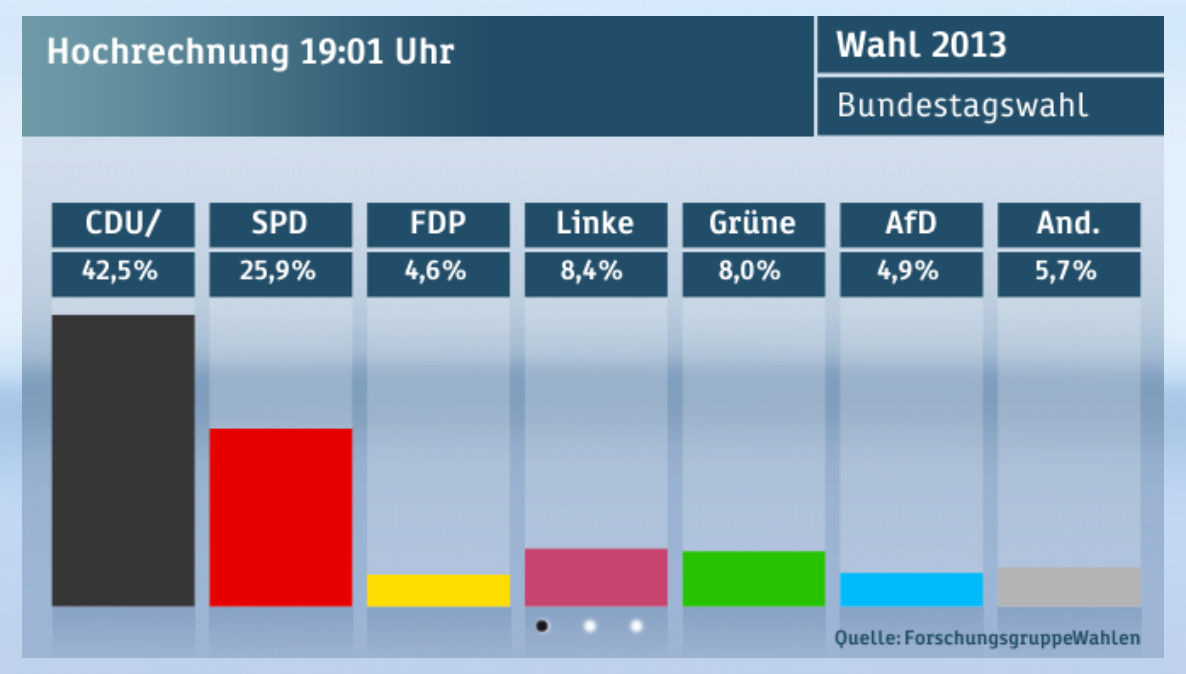
\includegraphics[scale=0.45]{ergebniswahl.png}
		\caption{Ergebnisse der Bundestagswahl 2013}
	\end{figure}
\end{frame}

\begin{frame}{Projekt - Aufgabenstellung}
	\begin{columns}[c] % the "c" option specifies center vertical alignment
  		\begin{column}[T]{0.4\textwidth} % each column can also be its own environment
			\textbf{Unser Ziel:}
			\begin{quote}
				``Visuelles Werkzeug zur Analyse und Auswertung von Wahlergebnissen in Bezug auf Einwohner- und Standortdaten."
			\end{quote}					
		\end{column}
		\begin{column}[T]{0.45\textwidth} % each column can also be its own environment
			\begin{figure}[hbtp]
				\centering
				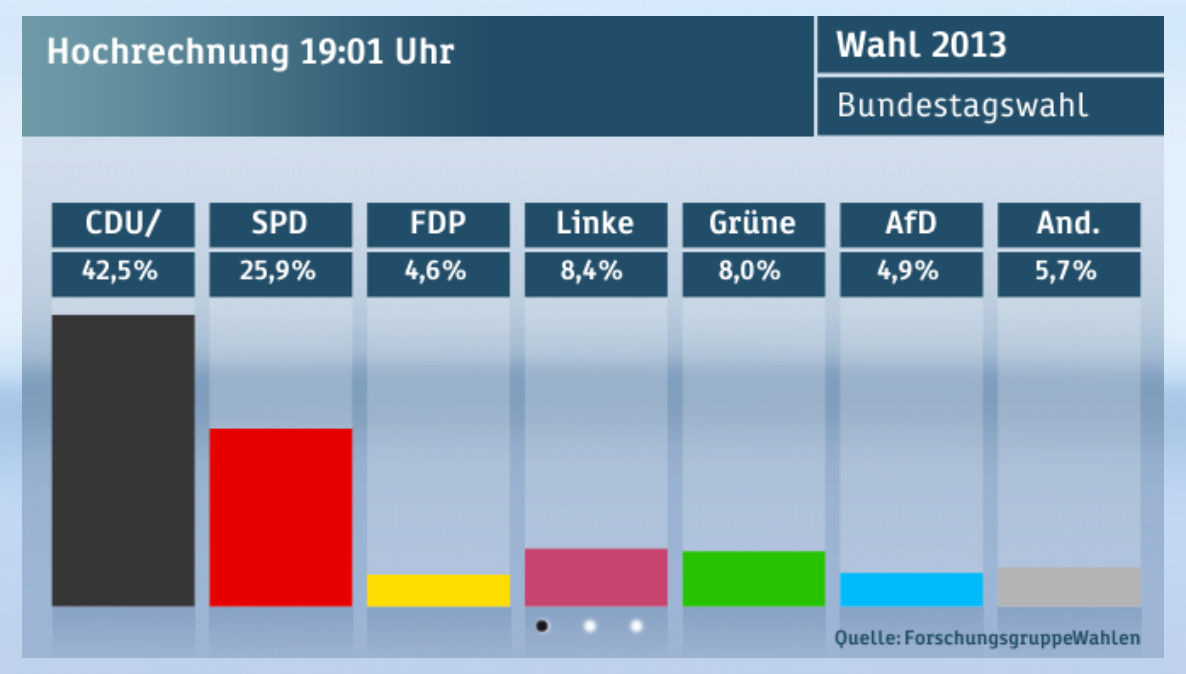
\includegraphics[scale=0.3]{ergebniswahl.png}
				\caption{Screenshot unserer Applikation}
			\end{figure}
  		\end{column}
  	\end{columns}
\end{frame}

\section{Projekt - Umsetzung}
\begin{frame}{Technologien}
	\begin{columns}[c] % the "c" option specifies center vertical alignment
  		\begin{column}[T]{0.49\textwidth} % each column can also be its own environment
			\textbf{Technologien}
			\begin{itemize}
				\item \href{http://www.java.com/en/}{Java} 
\includegraphics[scale=0.08]{javalogo.png}
				\item \href{http://www.postgresql.org/}{PostgreSQL} 
\includegraphics[scale=0.08]{postgresqllogo.png}
				\item \href{http://postgis.net/}{PostGIS} 
\includegraphics[scale=0.08]{postgislogo.png}
			\end{itemize}
		\end{column}
		\begin{column}[T]{0.49\textwidth} % each column can also be its own environment
			\textbf{Frameworks}
			\begin{itemize}
				\item \href{http://www.hibernatespatial.org/}{Hibernate Spatial} 
\includegraphics[scale=0.08]{hibernatelogo.png}
				\item \href{http://angularjs.org/}{AngularJS} 
\includegraphics[scale=0.05]{angularjslogo.png}
				\item \href{http://d3js.org/}{D3.js} 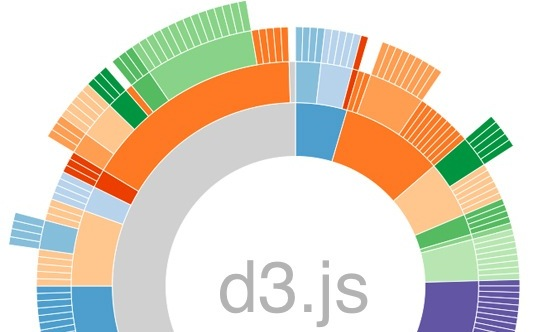
\includegraphics[scale=0.06]{d3jslogo.jpg}
				\item \href{http://getbootstrap.com/}{Twitter Bootstrap} 
\includegraphics[scale=0.08]{bootstraplogo.png}
			\end{itemize}
  		\end{column}
  	\end{columns}
\end{frame}

\begin{frame}{Datenmodell}
	\begin{center}
	\scalebox{.5}{
		\begin{tikzpicture}[node distance=1.5cm, every edge/.style={link}]

			\node[entity] (elec) {Election};
			\node[attribute] (elecId) [above=of elec] {\key{electionID}} edge (elec);
			\node[attribute] (elecDate) [above left=of elec] {date} edge (elec);

			\node[relationship] (hasE) [right=1cm of elec] {Has} edge node[auto,swap] {1} (elec);

			\node[entity] [right=1cm of hasE] (electionRes) {ElectionResult} edge node[auto,swap] {1...*} (hasE);
			\node[attribute] (electionResEId) [above=of electionRes] {\key{electionID}} edge (electionRes);
			\node[attribute] (electionResPId) [above right=of electionRes] {\key{partyID}} edge (electionRes);
			\node[attribute] (electionResPVotes) [above left=of electionRes] {Primary Votes} edge (electionRes);
			\node[attribute] (electionResSVotes) [below left=of electionRes] {Secondary Votes} edge (electionRes);
			
			\node[relationship] (hasP) [right=1cm of electionRes] {Has} edge node[auto,swap] {0...*} (electionRes);
			
			\node[entity] [right=1cm of hasP] (party) {Party} edge node[auto,swap] {1} (hasP);
			\node[attribute] (partyID) [above=of party] {\key{partyID}} edge (party);
			\node[attribute] (partyName) [above right=of party] {Name} edge (party);
			
			\node[relationship] (hasC) [below=1cm of electionRes] {Has} edge node[auto,swap] {0...*} (electionRes);			
			
			\node[entity] [below=1cm of hasC] (cons) {Constituency} edge node[auto,swap] {1} (hasC);
			\node[attribute] (consID) [left=of cons] {\key{constituencyID}} edge (cons);
			\node[attribute] (consName) [below left=of cons] {Name} edge (cons);
			\node[attribute] (consGeom) [below right=of cons] {Geom} edge (cons);
			
			\node[relationship] (hasCD) [right=1cm of cons] {Has} edge node[auto,swap] {1} (cons);
			
			\node[entity] [right=1cm of hasCD] (consData) {ConstituencyData} edge node[auto,swap] {1...*} (hasCD);
			\node[attribute] (consDataKey) [above=of consData] {Key} edge (consData);
			\node[attribute] (consDataValue) [above right=of consData] {Value} edge (consData);
			
			\node[relationship] (hasCo) [below=1cm of cons] {Has} edge node[auto,swap] {0...*} (cons);
			
			\node[entity] [below=1cm of hasCo] (county) {County} edge node[auto,swap] {1} (hasCo);
			\node[attribute] (countyID) [left=of county] {\key{countyID}} edge (county);
			\node[attribute] (countyName) [below left=of county] {Name} edge (county);
			\node[attribute] (countyGeom) [below right=of county] {Geom} edge (county);
			
			\node[relationship] (hasCoD) [right=1cm of county] {Has} edge node[auto,swap] {1} (county);
			
			\node[entity] [right=1cm of hasCoD] (countyData) {CountyData} edge node[auto,swap] {1...*} (hasCoD);
			\node[attribute] (countyDataKey) [above=of countyData] {Key} edge (countyData);
			\node[attribute] (countyDataValue) [above right=of countyData] {Value} edge (countyData);
			
		\end{tikzpicture}
	}
	\end{center}
\end{frame}

\begin{frame}{Architektur}

\end{frame}

\begin{frame}[fragile]{Beispielcode}
 	\begin{lstlisting}
		var width = 800, height = 600; // size of map
		var projection = d3.geo.mercator() // type of projection
        	.center([10.45, 51.16]) // center of Germany
        	.scale(2500)
        	.translate([width/2,height/2]);

		var coordinateWGS84 = [13.38, 52.52]; // Berlin
		var coordinateCartesian = projection(coordinateWGS84);

		=> coordinateCartesian = [377.85, 153.95]
  \end{lstlisting}
\end{frame}

\begin{frame}{Designentscheidungen}
	
\end{frame}

\section{Demo}
\begin{frame}{Demo}
	\begin{center}
		\huge Demo	
	\end{center}
\end{frame}


\end{document}
